% =============================================================================
% cs-memory-stack-heap.tex — Process memory layout with a heap pointer
%
% Shows: the classic process address-space picture — text / data / heap growing
% up, stack growing down — with a stack variable holding a pointer into a
% heap-allocated block.
% Compiles standalone via: xelatex cs-memory-stack-heap.tex
%
% Use for: data structures (malloc/free, pointers), operating systems, systems
% programming, and any "where does this variable actually live?" explanation.
%
% This is the diagram behind the CS301 Week 1 stack/heap traces — to build a
% step-by-step trace, copy this file once per step and change only the cells
% that the step modifies, keeping every coordinate identical between steps.
% =============================================================================

\documentclass[border=5pt]{standalone}
\usepackage{tikz}
\usetikzlibrary{arrows.meta, positioning}

\definecolor{seg-border}{HTML}{012169}
\definecolor{stack-fill}{HTML}{E8EDF5}
\definecolor{heap-fill}{HTML}{FDF6E8}
\definecolor{static-fill}{HTML}{F2F2F2}
\definecolor{ptr}{HTML}{B9975B}
\definecolor{muted}{HTML}{525252}
\definecolor{grow}{HTML}{15803D}

\tikzset{
  seg/.style={
    draw=seg-border, thick, minimum width=3.4cm, align=center, font=\small
  },
  addr/.style={font=\scriptsize, text=muted},
  ptr-edge/.style={-{Latex[length=2.4mm]}, thick, draw=ptr},
  grow-edge/.style={-{Latex[length=2.2mm]}, thick, draw=grow},
  note/.style={font=\scriptsize, text=muted, align=left}
}

% -----------------------------------------------------------------------------
% Diagram: address space drawn with HIGH addresses at the TOP (the usual
% textbook convention). Single column at x = 0, width 3.4cm.
% Coordinates: (x, y) — each segment is a box of stated height, stacked.
%   Stack   box centred (0,  2.60), height 1.6   [high addresses]
%   (gap: unallocated)            y in [0.95, 1.80]
%   Heap    box centred (0,  0.30), height 1.7
%   Data    box centred (0, -1.10), height 0.9
%   Text    box centred (0, -2.10), height 0.9   [low addresses]
% Growth arrows sit in the OUTER margin at x = 2.6 (right of the 1.7cm
% half-width), so they never overlap a box (P7a). Address labels sit at
% x = -2.3, left of the boxes. The heap pointer arrow runs from the stack
% variable's right edge, around through x = 2.15, down into the heap block —
% clear of both boxes.
% -----------------------------------------------------------------------------

\begin{document}
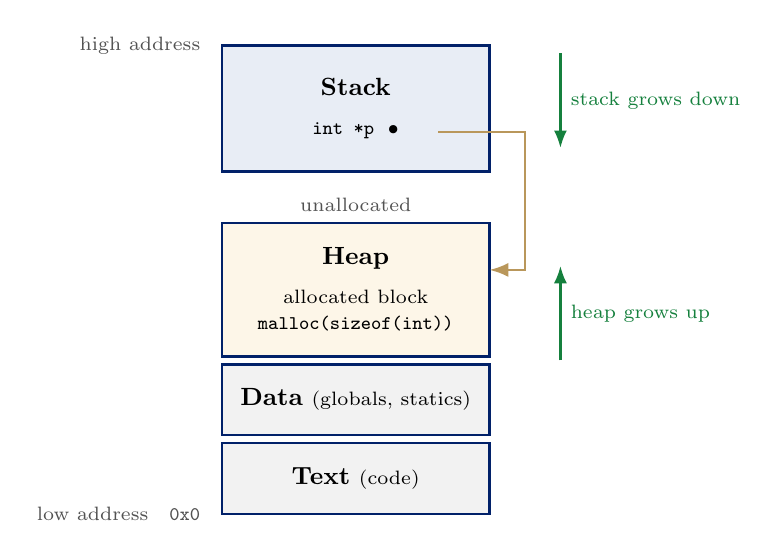
\begin{tikzpicture}

  % ---- Segments ------------------------------------------------------------
  \node[seg, fill=stack-fill,  minimum height=1.6cm] (stack) at (0,  2.60)
        {\textbf{Stack}\\[0.1cm]\scriptsize \texttt{int *p} \;$\bullet$};
  \node[seg, fill=heap-fill,   minimum height=1.7cm] (heap)  at (0,  0.30)
        {\textbf{Heap}\\[0.1cm]\scriptsize allocated block\\[-0.05cm]
         \scriptsize \texttt{malloc(sizeof(int))}};
  \node[seg, fill=static-fill, minimum height=0.9cm] (data)  at (0, -1.10)
        {\textbf{Data} \scriptsize (globals, statics)};
  \node[seg, fill=static-fill, minimum height=0.9cm] (text)  at (0, -2.10)
        {\textbf{Text} \scriptsize (code)};

  % ---- Unallocated gap between heap and stack -----------------------------
  \node[note, text=muted] at (0, 1.38) {\scriptsize unallocated};

  % ---- Address labels (left margin) ---------------------------------------
  \node[addr, left] at (-1.85,  3.40) {high address};
  \node[addr, left] at (-1.85, -2.55) {low address \; \texttt{0x0}};

  % ---- Growth-direction arrows (right margin, clear of the boxes) ---------
  \draw[grow-edge] (2.6,  3.30) -- (2.6,  2.10)
        node[midway, right, font=\scriptsize, text=grow] {stack grows down};
  \draw[grow-edge] (2.6, -0.60) -- (2.6,  0.60)
        node[midway, right, font=\scriptsize, text=grow] {heap grows up};

  % ---- Pointer from the stack variable into the heap block ----------------
  \draw[ptr-edge] (1.05, 2.30) -- (2.15, 2.30) -- (2.15, 0.55) -- (1.70, 0.55);

\end{tikzpicture}
\end{document}
